\label{sec:l2}
Die paarweise Kollisionserkennung bezieht sich auf die Kollision von konkret zwei 3D-Modellen. In diesem Schritt ist die Genauigkeit der Kollision bei steigender Modellkomplexität im Fokus.
Ziel ist es die Diskrepanzen zwischen der grafischen Anzeige von Modellen und der physikalischen Simulation zu deckeln.
\subsection{Input}
Aus dem vorhergehenden Schritt der Kollisionspaarermittlung werden für den Schritt der paarweisen Kollisionserkennung bis zu  $|OBJ|^2$ Objektpaare $C_{guess}\subseteq OBJ^2$ erhalten, für die eine Kollisionsvermutung während eines Ticks gilt. Man geht weiter davon aus, dass die Menge der tatsächlichen Kollisionen $C_{definitive}\subseteq OBJ^2$ in der Menge der vermuteten Kollisionspaare  vollständig enthalten ist $C_{definitive}\subseteq C_{guess}$, d.h. keine tatsächlichen Kollisionspaare im Paarermittlungsprozess verloren gehen. 

\subsection{Output}
Es ist eine Aufgabe dieses Schritts, die Reduzierung von $C_{guess}$ auf $C_{defintive}$ zu vollenden.\\
Eine zweite Aufgabe ist die Ermittlung von Informationen über den Hergang der Kollisionen der Paare in $C_{defintive}$.
Im Abschnitt~\ref{sec:usages} werden einige Verwendungszwecke der Kollisionsermittlung aufgelistet. 
Elemente der Aufzählung haben unterschiedliche Anforderungen hinsichtlich benötigter Information über den Kollisionsvorgang um realisiert werden zu können.

\begin{enumerate}
	\item Schnitt\\
		Die Frage ob Objekte $o_0,o_1 \in OBJ$ sich an einem konkreten Zeitpunkt während eines Ticks $t\in \Upsilon_{\delta i}$ schneiden/gegenseitig enthalten. $K_{o_0, t} \cap K_{o_1, t} \neq \emptyset$.
	\item Intrusion\\
		Die Frage nach den Eigenschaften
		\begin{enumerate}
		\item ob
		\item wann
		\item an welcher Raumposition
		\item mit welchen Teilen des Objektes
		\end{enumerate}
		ein Eindringen eines Objektes in ein anderes stattfindet, d.h. ein Zustandsübergang von Nicht-Kollision zu Kollision stattfindet.
		Der durchsuchte Zeitraum ist dabei eine kontinuierliche Schlusspartition der Ticksequenz $\Upsilon_{part} = \langle t_{searchstart}, ..., t_1 \rangle : (\Upsilon_{\delta i}\backslash \Upsilon_{part}) \smallfrown \Upsilon_{part} = \Upsilon_{\delta i} $ ($\smallfrown$ ist Konkatenation von Sequenzen) zu der relativ bei Zeitpunkt $j \in \Upsilon_{part} \subseteq \Upsilon_{\delta i}$ eine Erstkollision auftritt.\\
		So können nach dem finden der Erstkollision prinzipiell durch das verschieben von $t_{searchstart}$ noch weitere Erstkollisionen während des Ticks $\delta_i$ ermittelt werden.
		$$\exists j \in [1, |\Upsilon_{part}|-1], t_c= \Upsilon_{part}(j):$$
		$$ G_{o_0, t_c}\cap G_{o_1, t_c} \neq \emptyset \wedge \forall j' < j: 
		G_{o_0, \Upsilon_{part}(j')}\cap G_{o_1, \Upsilon_{part}(j')} = \emptyset$$
		Aus der Schnittmenge $G_{o_0, t_c}\cap G_{o_1, t_c}$ können dann die Angeforderten Eigenschaften zur Kollision (Zeit, Ort, Beteiligte Objektteile) ermittelt werden.
\end{enumerate}
Es mag weitere Forderungen an Kollisionsalgorithmen geben. Die obige Aufzählung stellt dabei die in dieser Arbeit in Betracht gezogenen dar.

Für physikalische Verwendungszwecke insbesondere bei der rigiden Objektkollision erscheint Intrusion besonders interessant. In Simulationen mit rigiden Kollisionsobjekten ist typischerweise der Zustand des Schnitts zweier Objekte nicht erlaubt und muss daher aktiv durch eine Kollisionsreaktion verhindert werden. Durch die Ermittlung des ersten Zeitpunkts des Bruchs der Nicht-Überschneidungsbedingung kann die Kollisionsreaktion passend ermittelt werden.\\
Die Umsetzung der Auflösung von Kollisionen und Mehrfachkollisionen ist explizit aus diesem Projekt ausgeschlossen. Selbst jedoch bei der theoretischen Betrachtung von Mehrfachkollisionen während eines Ticks und Optionen zu deren Auflösung, bzw.~physikalischer Reaktion von Objekten , scheinen vorwiegend Erstkollisionen interessant zu sein. Man vergleiche hierzu Abbildung~\ref{fig:l3col}.\\
An dieser Stelle wird demnach die Annahme getroffen, dass zunächst nur Erstkollisionen durch Intrusion interessanter sind sind und zuerst ermittelbar gemacht werden sollten.


%%TODO look if one can fit that under his hat somewhere, would be rad 
%Ein interessanter Fehler bezogen auf L3 in freier Wildbahn ist in \cite{skyrimwallglitch} zu sehen. Es handelt sich dabei um einen Glitch im Spiel The Elder Scrolls V:Skyrim. Dabei wird eine gleichzeitige Kollision des Spielermodells (welches sich durch eine Ingame-Fähigkeit unüblich schnell bewegt), eines Objekts und einer Wand oder Tür provoziert. Die Kollision, bzw. die wiederholten Kollisionen zwischen dem Spielermodell, dem Objekt (Kessel/Teller/Korb) und der Wand/Tür werden nicht richtig aufgelöst, was dazu führt, dass der Spieler durch die Wand laufen kann.\\


\subsection{Intrusionsermittlung durch lineare Interpolation der Objektbewegung}
\label{sec:linear_int}
Um das Problem zu vereinfachen wird die zunächst die Rotation von Objekten vernachlässigt.\\
Genauer: In diesem Kontext erfährt ein Objekt $o\in OBJ$ während eines Ticks $\delta_i$ keine zeitliche Änderung der Rotation $\forall t \in \Upsilon_{\delta i} : \omega(o, t) = (0,0,0)$. Dies hat mehrere Gründe:
\begin{enumerate}
\item Objekte hielten zum Start des Projekts noch keine Repräsentation für Rotation.
\item Rotation mit einzubeziehen wurde zu Anfang schon als schwierig eingestuft. Dieser Verhalt sollte sich später bestätigen.
\item Es gibt genügend Kollisionsszenarien/Verwendungszwecke für denen Rotation keine Rolle spielen muss. (Logische Kollision, Punktförmige Objekte, unbewegliche Objekte wie z.B. oft Terrain, Verwendungszwecke mit hoher Fehlertoleranz)
\item Es wird ein Experiment der Vernachlässigung von Rotation durchgeführt. Es soll dabei beantwortet werden, ob auch ohne Behandlung der Rotation eine ausreichend zufriedenstellende Illusion von physikalischem Realismus geschaffen werden kann.
\end{enumerate}

Wie in Abschnitt~\ref{sec:objects_sim} bereits beschrieben sind die zeitlichen Änderungen (Geschwindigkeit $v$ und Drehgeschwindigkeit $\omega$) eines Objektes während eines Ticks konstant. Durch die Vernachlässigung der Drehgeschwindigkeit $\omega$ kann die zeitliche Änderung eines Objektes $o$ allein auf Bezug zu Geschwindigkeit $v$ und der Zeit $t$ beschrieben werden, bzw.~alle im Objekt $o$ enthaltenen Punkte $p \in G_o$ beschreiben lineare, parallele Flugbahnen während des Ticks $\delta_i$:
$$l_p = \{p + (t - t_0) * v(o, t_0) | t_0 \leq t \leq t_1\}; X \subseteq \mathcal{F}^3:\{l_p|p\in X\} = \{X| t \in \Upsilon_{\delta_i}\}$$,
 die in ihrer Gesamtheit also das durchlaufene Volumen des Objekts beschreiben:
$$\{l_p|p\in G_o\} = \{G_{o, t}| t \in \Upsilon_{\delta_i}\}$$

Dies ermöglicht die Ermittlung von Kollisionen von Objekten $o_0, o_1$ durch lineare Interpolation der Zeit.\\
Die Eigenschaft der Linearität hat dabei noch den weiteren entscheidenden Vorteil, dass bei einer Relativierung der Objekte wechselseitig zueinander, eine Operation der einer Transformation in Form einer Translation gleichkommt, die Linearität weiterhin gewahrt bleibt. Zum Vergleich: Mit aktiver Rotation beschreiben Objekte relativ zueinander Kurvenflugbahnen.\\
Essenziell zu überprüfende Merkmalspaare $\in \{Area, Edge, Vertex\}^2$ sind:
		\begin{itemize}
			\item [$\{Vertex, Area\}$] Eine Ecke durchschlägt eine Fläche.\\
				$\Rightarrow$ Zu überprüfende Paare: $(V_{o_0}\times A_{o_1})\times (V_{o_1}\times A_{o_0})$
			\item [$\{Edge, Edge\}$] Kanten durchschneiden sich gegenseitig.
				$\Rightarrow$ Zu überprüfende Paare: $(E_{o_0}\times E_{o_1})\times (E_{o_1}\times E_{o_0}) = (E_{o_0}\times E_{o_1})$
		\end{itemize}
		Alle anderen Kombinationen sind entweder in diesen beiden enthalten (z.B. $\{Vertex, Edge\}$ in 1.) oder ein Ereignis dieser beiden Szenarien muss logisch vorher passieren (z.B. 1. oder 2. muss vor $\{Edge, Area\}$ bereits passiert sein).
\ \\
		Aufgrund der Relativierung muss nur eines der Merkmale muss eine zeitliche Bewegung durchführen
		\begin{itemize}
			\item [$$\{Vertex, Area\}$$] 2 Möglichkeiten:
				\begin{itemize}
					\item[Option0:] Eckpunkt $v \Rightarrow$ Linie $l_v$
					\item[Option1:] Dreiecksfläche $a \Rightarrow$ Schiefes Prisma $ \{l_p | p \in \mathcal{A}(a)\}$
				\end{itemize}
				Gewählt wird Option0, da einfachere Berechnung.
			\item [$\{Edge, Edge\}$] Kante $e \Rightarrow$ Parallelogramm $\{l_p | p \in \mathcal{E}(e)\}$
		\end{itemize}
\ \\
		Geometrische Eigenschaften nun beteiligter Formen:
		\begin{itemize}
			\item [Linie] $L = \{p_l | x\in\mathcal{F} ; p_{l0}, p_{l1} \in \mathcal{F}^3 ; p_l = p_{l0} + x * p_{l1}; 0\le x\le 1 \}$
		\item [Dreieck] $T = \{p_t | x,y \in\mathcal{F};  p_{t0},  p_{t1},  p_{t2} \in \mathcal{F}^3; p_t = p_{t0} + x*p_{t1} + y*p_{t2}; 0\le (x+y) \le 1\}$
			\item [Parallelogramm] $P = \{p_p | x,y \in\mathcal{F}; p_{p0}, p_{p1}, p_{p2} \in \mathcal{F}^3; p_p = p_{p0} + x*p_{p1} + y*p_{p2}; 0\le x\le 1; 0\le y\le 1\}$
		\end{itemize}
\ \\
		Beide Szenarien können über Gleichungssysteme zur Ermittlung von Ort- und Zeitkoeffizienten in konstanter Zeit überprüft werden:
		\begin{itemize}
			\item [$\{Vertex, Area\}$] $p_{l0} + x * p_{l1} = p_{t0} + y*p_{t1} + z*p_{t2}$\\
				$x$ ist zudem hier der Koeffizient der Zeit, da die Linie in der Zeitdimension liegt.
			\item [$\{Edge, Edge\}$] $p_{l0} + x * p_{l1} =  p_{p0} + y*p_{p1} + z*p_{p2}$\\
				Sei die ursprüngliche Kante, aus dem das Parallelogramm generiert wurde $\{p_0+y*p_1\}$, so liegt die andere Kante $\{p_0 + z*p_2\}$ in der Zeitdimension und somit ist hier z der Zeitkoeffizient.
		\end{itemize}
\ \\
		Komplexität: $\mathcal{O}(|V_{o0}|* |A_{o1}| + |V_{o1}|*|A_{o0}|$ + $|E_{o0}| * |E_{o1}|)$

		\begin{itemize}
			\item Zuverlässige Ermittlung der Erstkollision durch Findung des minimalen Zeitkoeffizienten.
			\item Mathematisch exakte Ermittlung der Zeit einer Kollision durch Zeitkoeffizienten.
			\item Mathematisch exakte Ermittlung des Orts einer Kollision durch Ortskoeffizienten.
			\item Ermittlung der Beteiligen Objektmerkmale der Erstkollision.
		\end{itemize}
Wie beschrieben kann dieses Verfahren bereits in einigen Szenarien, bei denen Rotation keine Rolle spielt, als vollständige Lösung zum Einsatz gebracht werden.\\
Es bleibt das Experiment, eine Illusion physikalischer Vorgänge mit rigider Körperkollision über den Linearen-Interpolationsalgorithmus zu realisieren.\\
Zunächst scheint dabei klar: Durch die Vernachlässigung der Rotation passieren physikungetreue Fehler, besonders, je größer die Varianz des Abstands der vom Objekt enthaltenen Punkte zum Objektursprung ist. Objekte sind dann unförmig und durchstreifen bei zeitlicher Bewegung logisch ein zu einem gewissen Grad anderes Volumen, als der lineare Interpolationsalgorithmus annimmt. Diese Diskrepanz kann sowohl zu False-Positives als auch zu False-Negatives führen.\\
Des Weiteren muss die vernachlässigte Rotation nachgeholt werden. Durch einen Extremfall dieser Nachlässigkeit fällt ein weiteres Defizit des Algorithmus auf. Ist die relative Geschwindigkeit zweier Objekte $=0$, wird aus Sicht des Algorithmus' kein Volumen durchstriffen. Es werden zwischen diesen Objekten dann gar keine Kollisionen erkannt, welche durch Rotation logisch/visuell aber auftreten.\\
Man versucht diese Problem durch statische Kollisionstests am Tickende zu lösen. Dabei wird die akkumulierte Rotationsbewegung/Rotationstransformation auf einmal ausgeführt. Vor und nach der Bewegung wird statisch eine Kollisionsabfrage berechnet.\\
Diese Anpassung bringt eigene Probleme mit sich:
\begin{enumerate}
\item Durch die akkumulierte Drehung kann eine Kollision bei schnellen Drehgeschwindigkeiten durch nur die Tests am Anfang und am Ende des Ticks komplett übersehen werden.
\item Nach der Rotationtransformation können Objekte sich in einem gegenseitigen Schnittzustand $D(o_0, t_1)\cap D(o_1, t_1) \neq \emptyset$ befinden, da an dieser Stelle keine Intrusion erkannt werden kann. Der Zustand könnte durch einen Linearen-Interpolationsalgorithmus zwar erkannt werden, jedoch sind bis dato im Projekt keine Möglichkeiten enthalten, vernünftig auf diesen Fall zu reagieren.
Eine Idee ist die Suche nach einem Zeitpunkt vor der Überschneidung, durch beispielsweise Bisection des Drehungsausschlags. Es erscheint jedoch, dass der wiederholte Aufwand durch Transformation und Ausführen des Interpolationsalgorithmus in der gegebenen Zeit ebenfalls keine Qualitativ hochwertigen Ergebnisse erzielt. Der Schnittzustand wird zudem in der rigiden Körperkollision als fehlerhafter Zustand angesehen, den die Kollisionsroutine eigentlich verhindern soll.
\end{enumerate}

%%TODO glitchpic

Es wird also weiter nach Lösungen gesucht, die sich dem Rotationsproblem besser annehmen.

\subsubsection{Gilbert-Johnson-Keerthi-Distanzalgorithmus (GJK)}
\label{sec:gjk}

\begin{figure}
\centering
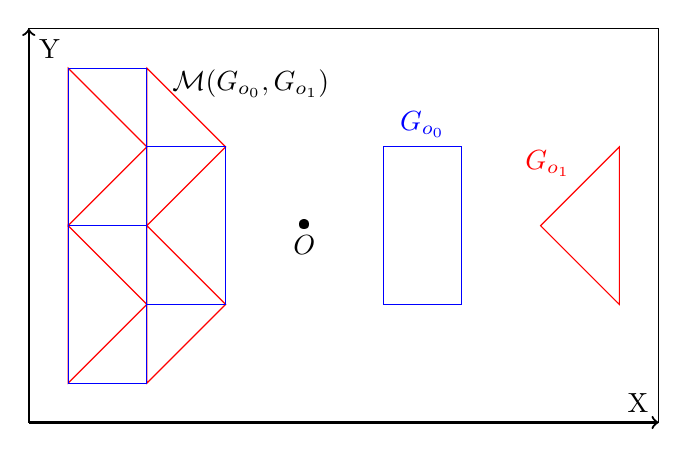
\begin{tikzpicture}

\draw (-3.5,-2.5) rectangle (4.5,2.5);
\draw[thick,->] (-3.5,-2.5) -- (4.5,-2.5) node[anchor=south east] {X};
\draw[thick,->] (-3.5,-2.5) -- (-3.5,2.5) node[anchor=north west] {Y};


\coordinate (O) at (0,0) ;
\draw [below](O) node[black]{$O$};
\draw (O) node[black]{\textbullet};

\coordinate (Ta) at (3, 0);
\coordinate (Tb) at (4, 1);
\coordinate (Tc) at (4, -1);

\draw[red] (Ta) -- node[above left]{$G_{o_1}$} (Tb) -- (Tc) -- cycle; 

\coordinate (Qa) at (1, -1);
\coordinate (Qb) at (1, 1);
\coordinate (Qc) at (2, 1);
\coordinate (Qd) at (2, -1);

\draw[blue] (Qa) -- (Qb) -- node[above]{$G_{o_0}$} (Qc) -- (Qd) -- cycle; 

\coordinate (QaTa) at (-2, -1);
\coordinate (QbTa) at (-2, 1);
\coordinate (QcTa) at (-1, 1);
\coordinate (QdTa) at (-1, -1);
\coordinate (QaTb) at (-3, -2);
\coordinate (QbTb) at (-3, 0);
\coordinate (QcTb) at (-2, 0);
\coordinate (QdTb) at (-2, -2);
\coordinate (QaTc) at (-3, 0);
\coordinate (QbTc) at (-3, 2);
\coordinate (QcTc) at (-2, 2);
\coordinate (QdTc) at (-2, -0);

\draw[red] (QaTa) -- (QaTb) -- (QaTc) -- cycle; 
\draw[red] (QbTa) -- (QbTb) -- (QbTc) --  cycle; 
\draw[red] (QcTa) -- (QcTb) -- (QcTc) -- cycle;
\draw[red] (QdTa) -- (QdTb) -- (QdTc) -- cycle;

\draw[blue] (QaTa) -- (QbTa) -- (QcTa) -- (QdTa) -- cycle; 
\draw[blue] (QaTb) -- (QbTb) -- (QcTb) -- (QdTb) -- cycle; 
\draw[blue] (QaTc) -- (QbTc) -- (QcTc) -- (QdTc) -- cycle; 

\node at (-1.8, 1.5)[above right]{$\mathcal{M}(G_{o_0}, G_{o_1})$};

\end{tikzpicture}
\caption{Beispiel für eine Minkowski-Differenz $\mathcal{M}(G_{o_0}, G_{o_1})$ mit Ursprung $O$ und den als Mesh angegebenen Objekten $G_{o_0}$ und $G_{o_1}$.}
\label{fig:gjk}
\end{figure}
GJK ist ein Algorithmus, der zwischen kompakten, konvexen Mengen $K_0, K_1 \subseteq \mathbb{R}^3$ die minimale euklidische Distanz $distance(K_0, K_1) = min\{|k_0 - k_1|~| k_0\in K_0 ; k_1 \in K_1\}$ errechnet. Er wurde 1988 publiziert \cite{gjk} und scheint heute gerne in Videospielen verwendet zu werden. Beispiele sind dabei Blizzard Entertainments Diabolo 3 \cite{gdc-physics} und Valves Half-Life 2\cite{gjk-casey}.\\
Die Urquelle \cite{gjk} beschreibt den Algorithmus umfassend mathematisch und ist daher aus unserer Sicht initial etwas schwere Kost. Es wird daher weiteres Quellmaterial \cite{gjk-casey} mit praktischerem Fokus zu Rate gezogen, um eine Implementierung umzusetzen und den Einstieg zu erleichtern.
Im GJK-Algorithmus sollen Eigenschaften der sogenannten Minkowski-Differenz $\mathcal{M}:\mathcal{P}(\mathbb{R}^3)^2\mapsto \mathcal{P}(\mathbb{R}^3); \mathcal{M}(K_0, K_1) = \{a - b| a\in K_0 ; b\in K_1\}$ \cite[p.195]{gjk} ausgenutzt werden. Ein Beispiel für die Minkowski-Differenz ist in Abbildung \ref{fig:gjk} zu sehen. Die hier relevanten Eigenschaften der Minkowski-Differenz lauten wie folgt:\\
	\begin{enumerate}
		\item Die Minkowski-Differenz zweier konvexer Körper ist ebenfalls konvex \cite[p.195]{gjk}.
		\item $K_0 \cap K_1 \neq \emptyset \Rightarrow \exists a_o, b_o \in K_0 \cap K_1, a_0 \in K_0, b_0 \in K_1 : a_o = b_o \Rightarrow a_o - b_o = O \Rightarrow O \in \mathcal{M}(K_0, K_1)$
		\item $K_0 \cap K_1 = \emptyset \Rightarrow \forall a_o\in K_0, \forall b_o\in K_1 : a_o \neq b_o \Rightarrow a_o - b_o \neq O \Rightarrow O \notin \mathcal{M}(K_0, K_1)$.
		\item $distance(O, \mathcal{M}(K_0, K_1)) = distance(K_0, K_1)$
		\item (2.) $\wedge$ (3.) $\wedge$ (4.) $\Rightarrow K_0 \cap K_1 \neq \emptyset \Leftrightarrow O \in \mathcal{M}(K_0, K_1)	\Leftrightarrow distance(K_0, K_1) = 0$	
		\item (4.) $\Rightarrow distance: \mathcal{P}(\mathbb{R}^3)^2 \mapsto \mathbb{R}^+_0$ (gibt nur positive Distanzen aus)
	\end{enumerate}
	Man bemerkt: Das Verfahren behandelt das Schnittproblem, statt des Intrusionsproblems. Durch die Fähigkeit des GJK-Algorithmus, die Distanz zwischen zwei Objekten zu ermitteln, ist dieser jedoch ein praktisches Werkzeug auch um das Intrusionsproblem ebenfalls zu lösen.
Zum Beispiel ist ein Ansatz mit GJK, durch Abstraktion über einer Nullstellensuche der Distanz zwischen zwei Objekten das Intrusionsproblem zu abzubilden (vgl.~Eigenschaft 5, vgl. \cite{gdc-physics}).\\
GJK eignet sich also für dieses Projekt und soll implementiert werden. 

Zunächst muss die Eingabeinformation von kompakten, konvexen Punktmengen, die der Algorithmus fordert, äquivalent hergestellt sein, um sicherzustellen, dass der Algorithmus auch mit Polygon-Meshes durchgeführt werden kann. Für diese ist allerdings keine Konvexität gefordert und eine entsprechende kompakte Repräsentation nicht gegeben.
Zunächst soll Konvexität hergestellt werden. Definierte nicht-konvexe Objekte können in Konvexe Partitionen aufgeteilt werden. Jede Partition zählt dann als eigenes Objekt gegenüber dem Algorithmus. Das erhöht die erwartete Komplexität der gesamten Kollisionsroutine mit GJK um den Grad der Partitionierung.\\
\ \\
Es wurde zu einer automatisierten Methode recherchiert, um die Partitionierung herzustellen. Insbesondere die minimale Partitionierung scheint hier von Interesse, um die Erhöhung der Komplexität zu mitigieren.\\
Zusätzlich zu eigenen Überlegungen bestätigen die Quellen \cite{ARTIGAS20111968} und \cite{grelier2019minimum} die NP-Vollständigkeit, bzw. NP-Härte zusammengehöriger Probleme der minimalen konvexen Partitionierung.\\
Eine nicht minimale Partitionierung wäre zunächst auch ausreichend und auch lange Berechnungszeiten zur Partitionierung würden für rigide Objekte nur einmaligen Aufwand zum Programmstart bedeuten und wären daher nicht kritisch.\\
Bei Versuchen, Algorithmen für dieses Problem zu erstellen, wird jedoch eine weiter klare Hürde erkenntlich: Allein durch die Polygon-Mesh, sind Innen und Außenseite des Objektes prinzipiell nicht definiert.\\
Für grafische Zwecke kann dieser Bezug oft durch das sog. \textit{Winding} eines Dreiecks angegeben werden. Dabei wird die Reihenfolge der Angabe der Ecken eines Dreiecks konventionell festgelegt, wodurch die Richtung der Flächennormale eines Dreiecks kontrolliert werden kann, die dann Außen oder Innenseite spezifiziert. Auch die direkte Angabe einer Flächennormale zu jedem Dreieck (oder sogar jedem Eckpunkt) is im graphischen Kontext für bestimmte Effekte gebräuchlich. Diese Konzepte werden grafisch im Projekt jedoch bis dato nicht verwendet und sind daher auch nicht vorhanden.\\
Eine Konvention für ein \textit{Winding} wurde allerdings im Projekt eingeführt, nicht zuletzt, da diese die Implementierung des GJK vereinfacht.\\
Für die in dieser Projektarbeit verwendeten Testzwecke erscheint der Aufwand der Automatisierung der konvexen Partitionierung für dieses Projekt letztendlich doch zu hoch und thematisch zu fremd.\\
\ \\
Die konvexe Partitionierung des Objektes $o$ wird daher manuell und explizit bei Modellen durch die Angabe von Mengen von Indices von zueinander konvexen Eckpunkten $P_o := \{P_0, ...\}; P_i \subseteq V_o$ angegeben.
Zusätzlich ist die Äquivalenz zur kompakten Punktemenge $K_o$ gefordert. Diese ist nun implizit durch die Konvexität gegeben. $K_o$ ist konvex, wenn gilt $\forall p_0, p_1 \in K_o, \forall x \in [0,1] : p0 + x * (p_1 - p0) \in K_o $. In Mesh-Repräsentation $G_o$ sind nicht alle diese Punkte enthalten. Jedoch, wenn $K_o$ konvex so sind die Hüllen $\mathcal{H}(K_o) = \mathcal{G_o}$ ebenfalls konvex. Alle Punkte $K_o \backslash G_o$ können so durch die Konvexitätsdefinition impliziert werden. Die zusätzlich mit der Objektrepräsentation mitgelieferte Partitionierung erweitert also die verfügbare Information und schafft in dieser Hinsicht Äquivalenz zwischen Polygon-Meshes und kompakten Mengen und die Unterscheidung von Innen und Außen. Informationen zu verbundenen Ecken einer Polygon-Mesh $I_o$ werden dadurch in diesem Kontext ebenfalls redundant. Der Algorithmus kann demnach außschließlich unter Einbeziehung von Eckpunkten $V_o$ verfahren.\\
Durch die Feststellung der Äquivalenz wurde ermittelt, dass eine Variante des GJK-Algorithmus auch an Polygon-Meshes durchgeführt werden kann.\\
Es kann also eine Diskretion/Beschränkung auf die Information der Eckpunkte der Polygon-Mesh $V_o$  verwendet werden, was vorteilhafte Iterationslängen im Algorithmus zur Folge hat ($V_o \ll G_o \ll K_o$).

%%TODO refactor and actually provide the images
Eine Illustation einer diskreten Minkowski-Differenz ist in den Abbildungen \ref{fig:minkov_col}, \ref{fig:minkov_col_solo} und \ref{fig:minkov_noncol}zu sehen. Zu sehen sind, in Rot und Blau, die 2 Objekte, welche sich in \ref{fig:minkov_col} überschneiden und in \ref{fig:minkov_noncol} nicht. Die Gebilde, deren Ecken grün sind und deren Kanten rot und blau sind sind die jeweiligen Minkowski-Differenzen.
Die grünen Punkte sind alle Punkte, die durch die Anwendung der Minkowski-Differenz auf die Menge der Eckpunkte beider Körper ermittelbar sind.\\
Die Kanten sind rot oder blau, je nachdem von welchem Ursprungskörper eine Kante Einfluss erhält. So ist die Beteiligung beider Körper an der Differenz besser zu erkennen. Theoretisch sind auch die Kanten zwischen jedem Punktepaar mit gemischten Einflüssen der beiden Ursprungsobjekte darstellbar, welche aus Darstellungsgründen nicht in der Grafik enthalten sind. Isoliert steht in Abbildung \ref{fig:minkov_col_solo} die Minkowski-Differenz aus Abbildung \ref{fig:minkov_col}.\\


Eigenschaften der Minkowski-Differenz müssen den Umstand der Diskretion respektierend ausgenutzt werden.\\

\begin{enumerate}
		\item Die diskrete Minkowski-Differenz ist ebenfalls konvex.	
		\item Ein Simplex ist eine durch eine Anzahl $n\in\mathbb{N}$ Eckpunkte $s\in\mathcal{M}(V_{o_0}, V_{o_1})^n$ aufgespannte $n$-dimensionale geometrische, inhärent konvexe Form (hier: Punkt für $n=1$, Gerade $n=2$, Dreieck $n=3$, Tetraeder $n=4$). Durch die Konvexität ist die entsprechende kompakte Menge $K_s$ implizit definiert.
		\item Für das nächste Simplex $s_{nearest} \in \mathcal{M}(V_{o_0}, V_{o_1})$ zum Ursprung $O$ gilt außerdem $distance(O, s_{nearest}) = distance(K_{o_0}, K_{o_1})$ \cite[p. 195]{gjk}. 
		\item $O \in \mathcal{M}(K_{o_0}, K_{o_1}) \nRightarrow O \in \mathcal{M}(V_{o_0}, V_{o_1})$. Jedoch kann eine äquivalente Beziehung gefunden werden: $O \in \mathcal{M}(K_{o_0}, K_{o_1}) \equiv \exists Simplex~s \in \mathcal{M}(V_{o_0}, V_{o_1}) : O \in K_s$, , das den Ursprung enthält/umschließt.

\end{enumerate}

Die Implementierung des GJK bezieht sich also auf die Suche nach dem nähersten, bzw. umschließenden Simplex zum Ursprung.\\
Es wird im Folgenden der Algorithmus beschrieben:
\begin{enumerate}
	\item Initialisiere mit
	\begin{enumerate}
		\item Zwei konvexen (Teil-)Objekten $o_0, o_1$
		\item ihrer diskreten Minkowski-Differenz zu einem Zeitpunkt $t$: $\mathcal{M} = \mathcal{M}(V_{o_0, t}, V_{o_1, t})$
		\item beliebigem Startpunkt $s_0 \in \mathcal{M}$
		\item der Menge von maximal 4 indizierten Simplexeckpunkten, wobei der Startpunkt bereits ein Simplex darstellt $s = \{s_0\}$
		\item der Suchrichtung $\vec{D} = -s_0$
		\item der minimalen gefundene Distanz $d_{min} = \infty$
		\item der Fähigkeit, Abstände zwischen einem Simplex und dem Ursprung zu errechnen $distance: Simplex \times \mathcal{F}^3 \mapsto \mathcal{F} ; distance({}, X) = \infty$
	\end{enumerate}	
	\item Finde neuen Punkt $s_{|s|}$ zur $(|s|+1)$-dimensionalen Erweiterung des Simplex den maximalen Punkt $v \in \mathcal{M}$ in der Suchrichtung $\vec{D}$ über das Skalarprodukt $s_{|s|} = v \in \mathcal{M} : \vec{v} \circ \vec{D} = max\{\vec{D} \circ \vec{v_i}| v_i \in  \mathcal{M}\}$. Da $\mathcal{M}$ konvex, existiert dieses Maximum in jede Richtung \cite[p. 195]{gjk}.
	\item $\vec{s_{|s|}} \circ \vec{D} < 0 \Rightarrow O \notin \mathcal{M}(K_{o_0, t}, K_{o_1, t})$. Es könnte $d_{min} = distance(s, O)$ gesetzt werden. Dieser Schritt ist hauptsächlich für einen verfrühten Abbruch interessant, wenn nur ermittelt werden soll, ob ein Schnitt $K_{o_0, t} \cap K_{o_1, t} \neq \emptyset$ existiert, oder nicht.
	\item Durch die Punkte $Simplex~s_{new} = s \cup {s_{|s|}}$ kann eine Menge von Simplices $\mathcal{P}(s_{new})$ beschrieben werden. Es soll das zum Ursprung nächste Simplex ausgewählt werden. Die Auswahl $\mathcal{P}(s_{new})$ kann weiter dadurch eingeschränkt werden, dass nur neue Simplices, die durch den neuen Punkt $s_{|s|}$ bekannt wurden überprüft werden müssen, da durch die Suche des Punkts in Suchrichtung $\vec{D}$ an dieser Stelle eine Distanzverbesserung durch den neuen Punkt erwartet wird. Das Gegenereignis hierzu kann durch Konvexität von $\mathcal{M}$ und der Maximaleigenschaft der Punkte in $s$ ausgeschlossen werden, solange das nächste Simplex nicht bereits erreicht ist \cite{gjk-casey}.  Die reduzierte Menge $S_{check} \subset \mathcal{P}(s_{new}); S_{check} = \{ s \in \mathcal{P}(s_{new}) | s_{|s|} \in s \}$ wird demnach stattdessen überprüft und das neue nächste gefundene Simplex 
	 $s \in s_{near} : s_{near} = \{\hat{s} | distance(\hat{s}, O) = min\{distance(s', O) | s' \in s_{check}\}\}; |s| \leq |\hat{s}| \in s_{near}$
	 ermittelt. Dabei haben die wenigerdimensionalen Simplices Vorrang bei Gleichheit.\\
	 In der Implementierung wird das durch geometrische Raumaufteilungen realisiert. So wird beim höchstdimensionalen Simplex $\dot{s}\in s_{check}: |\dot{s}| > |\ddot{s}|; \forall \ddot{s} \in s_{check}; \dot{s}\neq\ddot{s}$ begonnen und sukzessive festgestellt, in welchem zugehörigen Raumsegement von niedrigerdimensionalen Teilsimplices $\mathcal{P}(\dot{s})$ sich der Ursprung befindet. So beispielsweise zu einer Kante $\vec{s_{|s|}v}, v\in \dot{s}$ drei Raumsegmente gegeben. Zu den Endpunkten der Kante $\overline{s_{|s|},v}$ jeweils $SEG_{v} = \{p | p \circ \vec{s_{|s|}v} > 0\}$, bzw.  $SEG_{s_{|s|}} = \{p | p \circ \vec{vs_{|s|}} > 0\}$ und für die Kante selbst $\mathbb{F}^3 \backslash (SEG_{s_{|s|}} \cup SEG_{v})$, die alle Punkte beinhaltet, zu denen ein orthogonaler Vektor zur Geraden $\overline{s_{|s|},v}$ angegeben werden kann. Dabei kann die Überprüfung von $SEG_v$ ausgeschlossen werden, da $\{v\} \notin s_{check}$.
	 Die Zugehörigkeit des Ursprungs zu einem Segment kann durch Skalar- und Kreuzprodukte festgestellt werden. Genauere Angaben, sowie die Umsetzung von anderen Arten von Simlices (z.B. Dreiecke) behandelt die Quelle \cite{gjk-casey} ausführlicher.
	\item Falls keine kleineren Distanz gefunden wurde, ist das nächste Simplex zum Ursprung gefunden. $d_{min} \leq distance(s, O) \Rightarrow distance(K_{o_0}, K_{o_1}) = distance(s, O) = d_{min}$ (\textbf{RETURN})
	\item Ist das nächste Simplex ein Tetraeder $|s| = 4 \Rightarrow O \in K_s \Rightarrow distance(\mathcal{M}, O) = 0$ (\textbf{RETURN})
	\item $d_{min} = distance(s, O)$
	\item Die neue Suchrichtung $\vec{D} = D_{new}(s)$ wird orthogonal zum Simplex $s$ in Richtung des Ursprungs festgelegt. Die konkrete Berechnung hängt dabei von der Form des Simplex, also von $|s|$, ab. Ein Beispiel ist: $|s| = 2 \Rightarrow D_{new}(s) = (b-a)\times (O-a)\times (b-a);  \{a, b\} = s$, mit $\times$ als Kreuzprodukt zweier Vektoren.
	\item Wiederhole ab 2.
\end{enumerate}
Rückgabewerte sind immer $d_{min}$ \& $s$.
Es werden im Folgenden relevante Implementierungsspezifika und aufgetretene Probleme geschildert:\\
\begin{enumerate}
\item Für die Berechnung von Minkowski-Punkten $\mathcal{M}(V_{o_0}, V_{o_1})$ wurde ein Generator implementiert, der zum Minkowski-Punkt die Indices der Verwendeten Eckpunkte der Ursprungsmodelle $V_{o_0}$ und $V_{o_1}$ mitführt. Damit können durch den Erhalt des nächsten Simpex $s$ die Beteiligten Merkmale/Simplices and den Ursprungsobjekten ermittelt werden.
\item Die Quelle \cite{gjk-casey} ist zunächst primär für die Struktur des Implementierungsversuchs. Die dort gezeigte Implementierung funktioniert angeblich alleinig auf Basis der Abbruchkriterien in 3.~(verfrühter Abbruch) und 6.~ ohne 5..
Die Grafik \ref{fig:why_criteria} zeigt dabei einen Widerspruch, dass das vorgeschlagene Abbruchkriterien in 3. und 6. nicht ausreicht um ein nächstes Simplex zum Ursprung zu erreichen und die minimale Distanz zu ermitteln.\\
Unter Umständen ist es die undokumentierte Intention der Quelle \cite{gjk-casey} nur eine Implementierung zu liefern, die keine minimale Distanz oder nächste Simplices ermittelt, sondern nur ob ein Schnitt existiert, oder nicht. Die Ausschreibungen der Quelle als Implementierung des GJK-Algorithmus ist daher etwas irreführend, erleichterte jedoch den Einstieg in die Materie.
\item Die ungenügende Implementierung wurde daraufhin auf die Anforderungen von Distanz- und Simplexfindung unter Zuhilfenahme von Quelle \cite{gjk} angepasst.
Bei der Anpassung wurde zunächst mit Abbruchkriterien experimentiert um den im Schritt 4.~gezeigten Brute-Force-Aufwand der minimalen Distanzberechnungen zu vermeiden. Vorschläge sind:
\begin{enumerate}
	\item Die hier als Status-Quo vorgestellte Brute-Force-Distanzberechnung in Schritt 4.~und anschließende Auswertung in Schritt 5..
	\item Statt Schritt 5.:
	 $$s_{|s|} \in s \Rightarrow distance(K_{o_0}, K_{o_1}) = distance(s, O) = d_{min}\text{(\textbf{RETURN})}$$ 
	 Neue Simplexpunkte $s_{|s|}$ sind nach Schritt 2.~ maximal in einer Suchrichtung $D$, die in Richtung des Ursprungs liegt und liegt daher in der konvexen Objekthülle. Ist das nächste Merkmal erreicht, so wird nach Schritt 4.~in eine Richtung gesucht, deren maximale Punkte bereits bekannt sein müssen. Daher ist ein mögliches Abbruchkriterium: Abbruch beim finden eines Support-Punktes, der bereits bekannt ist. $\mathcal{O}(3)$, da in Schritt 4.~immer gilt $|s|\leq 3$ und Suchrichtungen $D$ immer orthogonal gewählt werden.
	\item Durch den neuen Punkt $s_{|s|}$ gezogene Kantenvektoren $\vec{s_{|s|}v}, v\in s$ sollen eine klare Erweiterung in Suchrichtung $\vec{D}$ darstellen, was durch $\vec{D} \circ \vec{s_{|s|}v} < 0$ ermittelbar ist. Diese Kriterium soll nur dann geprüft werden, wenn durch Schritt 3. bereits ermittelt wurde, dass der Ursprung außerhalb des Suchkörpers liegt und die Punkte in $s$ bereits auf der Seite des Suchkörpers liegen, an der sich der Ursprung angrenzt.
\end{enumerate}

\begin{figure}
	\centering
	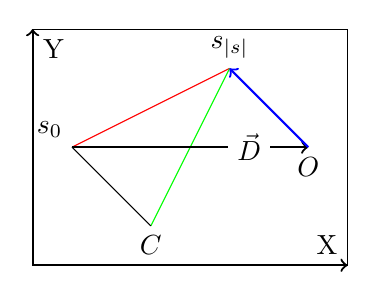
\begin{tikzpicture}
	\draw (-3.5,-1.5) rectangle (0.5,1.5);
	\draw[thick,->] (-3.5,-1.5) -- (0.5,-1.5) node[anchor=south east] {X};
	\draw[thick,->] (-3.5,-1.5) -- (-3.5,1.5) node[anchor=north west] {Y};

	\coordinate (A) at (-1,1);
	\coordinate (B) at (-3,0);
	\coordinate (C) at (-2,-1);
	\coordinate (O) at (0,0);

	\draw [red] (B) node[black, above left]{$s_0$} -- (A) node[black, above]{$s_{|s|}$};
	\draw [green] (A) -- (C)  node[black, below]{$C$};
	\draw (C) -- (B);
	\draw [thick, ->] (-3,0) -- (0,0) node [near end,fill=white]{$\vec{D}$} node [below] {$O$};
	\draw [thick, blue, ->] (O) -- (A);
	\end{tikzpicture}
	\caption{Szenario für fehlerhaftes Abbruchkriterium aus \cite{gjk-casey} nicht am nächsten Merkmal zum Ursprung stoppt. Startpunkt $s_0$, maximaler Punkt in $\vec{D}$ ist $s_{|s|}$, stopp nach Schritt 3. mit (rot) $s_{new} = \{s_o, s_{|s|}\}$, da (blauer) Vektor $\vec{s_{|s|}}\circ\vec{D} < 0$. Tatsächliches nächstes Simplex zu $O$ ist aber (grün) $\overline{s_{|s|}C}$.}
	\label{fig:why_criteria}
\end{figure}

\begin{figure}
	\centering
	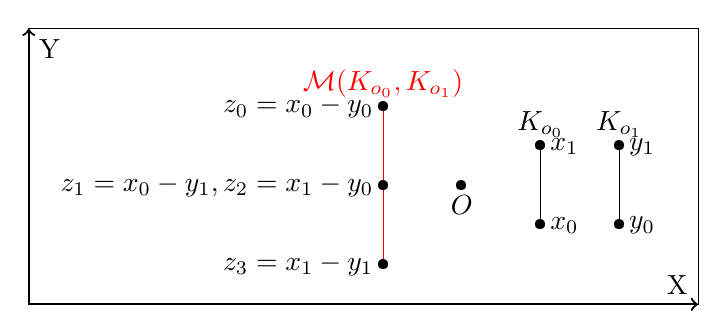
\begin{tikzpicture}



\draw (-5.5,-1.5) rectangle (3,2);
\draw[thick,->] (-5.5,-1.5) -- (3,-1.5) node[anchor=south east] {X};
\draw[thick,->] (-5.5,-1.5) -- (-5.5,2) node[anchor=north west] {Y};

\coordinate (VOaa) at (1,-0.5);
\coordinate (VOab) at (1,0.5);
\coordinate (VOba) at (2,-0.5);
\coordinate (VObb) at (2,0.5);

\coordinate (O) at (0,0);

\coordinate (A) at (-1,0);
\coordinate (B) at (-1,1);
\coordinate (C) at (-1,-1);

\draw [below](O) node[black]{$O$};
\draw (VOaa) -- (VOab);
\draw (VOba) -- (VObb);
\draw [red] (A) -- (B) -- (C);

\node at (O) {\textbullet};
\node at (A) {\textbullet};
\node at (B) {\textbullet};
\node at (C) {\textbullet};
\node at (VOaa) {\textbullet};
\node at (VOab) {\textbullet};
\node at (VOba) {\textbullet};
\node at (VObb) {\textbullet};

\node at (VOab)[above] {$K_{o_0}$};
\node at (VObb)[above] {$K_{o_1}$};

\node at (VOaa) [right]{$x_0$};
\node at (VOab) [right]{$x_1$};
\node at (VOba) [right]{$y_0$};
\node at (VObb) [right]{$y_1$};

\node at (B) [above, red]{$\mathcal{M}(K_{o_0}, K_{o_1})$};


\node at (B) [left]{$z_0=x_0-y_0$};
\node at (A) [left]{$z_1=x_0-y_1, z_2=x_1-y_0$};
\node at (C) [left]{$z_3=x_1-y_1$};

\end{tikzpicture}
	\caption{Minkowski-Differenz (rot) $\mathcal{M}(K_{o_0}, K_{o_1})$ mit markierten Punkten $\mathcal{M}(V_{o_0}, V_{o_1})$ mit mehreren nächsten Simplices $\{ \{z_1\},\{z_2\},\{z_0, z_3\},\{z_0,z_1\},\{z_1,z_2\}, ...\}$ zum Ursprung, sogar inklusive zweier deckungsgleicher 1D Simplices mit kleinster Dimensionalität 1.}
	\label{fig:parfeat}
\end{figure}

Bei Versuchen mit den Abbruchkriterien (b) und (c) konvergierte der Algorithmus regelmäßig nicht. Es wurden falsche Annahmen getroffen:
\begin{enumerate}
\item Das nächste Simplex zum Ursprung ist eindeutig.\\
Die Minkowski-Summe produziert keine Hüllenobjekte, nur konvexe Vertex-Meshes. Es können daraus mehrere nächste Simplices zum Ursprung generiert werden, wie die Abbildung \ref{fig:parfeat} zeigt. Das Problem kann dann auftreten, wenn Simplices in (denselben oder gepaarten) Ursprungsmerkmalen komplanar sind.
\item Verwendete Funktionen sind ausreichend genau.\\
Theoretisch sollten komplanare Merkmale dieselbe neue Suchrichtung $\vec{D}$ in Schritt 8.~erzeugen. Der neue Punkt $s_{|s|}$ ist dabei dann eindeutig (maximales Skalarprodukt im Konvexen). Das scheint durch Berechnungsungenauigkeiten, insbesondere im Kreuzprodukt, nicht der Fall zu sein. 
\end{enumerate}

Die Uneindeutigkeit der nächsten Simplices und Berechnungsungenauigkeiten führten im Algorithmus zu wiederholt denselben Belegungen von $s$ und somit zu Endlosschleifen.\\
Nur Abbruchkriterium (a) arbeitet nicht mit dem Kreuzprodukt, führte in allen Tests immer erfolgreich zur Konvergenz und wird daher letztendlich verwendet.
\end{enumerate}

~\\
GJK löst so das Schnittproblem zu einem Zeitpunkt $t$. Über die Suche der ersten Nullstelle des GJK als Distanzfunktion während eines Ticks kann die Zeit einer Erstkollision bestimmt werden, um zusätzlich das Intrusionsproblem zu lösen.
Ein Nullstellen-/Wurzelsuchverfahren hat zudem den Vorteil, dass es unabhängig von der Bewegungsart der Objekte ist. Animation, Rotation oder beliebige Transformation ist prinzipiell denkbar, solange die Bewegung und damit die Distanz stetig ist.\\
Es sind prinzipiell viele Wurzelsuchverfahren bekannt. Viele werden jedoch durch den Umstand einer niemals negativen Distanz $\Rightarrow distance: \mathcal{P}(\mathbb{R}^3)^2 \mapsto \mathbb{R}^+_0$ verkompliziert. Eine negative Distanz, also eine Penetrationstiefe, berechenbar zu machen würde die Implementation des GJK-Algorithmus allerdings weiter verkomplizieren.\\


Vor allem im Falle von rotierenden Objekten werden Hürden ersichtlich:
Bei Rotierenden Objekten nimmt die Distanzfunktion die Form einer Schwingung an, wodurch das Nyquist-Shannon-Abtasttheorem gilt. Die korrekte Ermittlung der Erstkollision im Rahmen eines Ticks kann durch Aliasing besonders bei schnellen Rotationen prinzipiell verhindert werden. Es gilt also auch bei diesem Verfahren eine Einschränkung der Rotationsgeschwindigkeit oder Verlust des 100\%-igen Erfolgs des Verfahrens. Es bestätigt sich hier wieder die bereits in Abschnitt~\ref{sec:linear_int} gemachte Einschätzung von Rotation als limitierenden Faktor. Anders als bei der linearen Interpolation kann bei diesem Verfahren jedoch besser auf die Limitation eingegangen werden. Unter Einbeziehung weiterer Information der kollidierenden Objekte, z.B. Rotationsgeschwindigkeit, Varianz können Wurzelsuchverfahren ausgewählt und ihre Parameter angepasst werden.\\
Es wurde ein Verfahren implementiert, welches zunächst mit einer einstellbaren Abtastrate $r_{sample}$  pro Ticks nach einer Distanz $= 0$ sucht. Das erste zeitliche Auftreten eines solchen Ereignisses wird dann weiter zur Bisektion des durch Samples eingegrenzten Zeitabschnitts verwendet, um den bei der Intrusion geforderten Zeitpunkt mit einer bestimmten Genauigkeit $\epsilon_t$ festzustellen.\\

Die Komplexität des Verfahrens hängt von den Komplexitäten der Teilalgorithmen ab:
\begin{enumerate}
\item die Anzahl der konvexen Partitionen der Objekte $\mathcal{O}(|P_{o_0}|*|P_{o_1}|)$
\item der Komplexität des Wurzelsuchverfahrens:\\
 Für das in diesem Projekt verwendete Verfahren ist dies $$\mathcal{O}(r_{sample} + \log_{2}(\frac{(t_1 - t_0)}{r_{sample}\epsilon_t} )$$
\item der Komplexität von GJK:\\
Ein Durchlauf der in Schritt 9.~angelegten Schleife bringt die Komplexität der Zwischenschritte mit sich. Die nicht-trivial Konstanten sind:
\begin{enumerate}
\item Schritt 2.: $\mathcal{O}(|\mathcal{M}(V_{o_0}, V_{o_1})|) = \mathcal{O}(|V_{o_0}|*|V_{o_1}|)$.
Die Urquelle \cite[p.196, Mathindex 16, 17, 21]{gjk} beschreibt die Optimierung auf $\mathcal{O}(|V_{o_0}|+|V_{o_1}|)$. Diese ist in dieser Implementierung noch nicht enthalten.
\item Schritt 4.: $\mathcal{O}(\mathcal{P}(s)) = \mathcal{O}(2^{|s|})$, aber $|s| \leq 4 \Rightarrow \mathcal{O}(2^4) = \mathcal{O}(16)$. Außerdem ist 
\end{enumerate}
Die Komplexität innerhalb der Schleife hängt also hauptsächlich von der Beschaffenheit der Objekte, bzw.~ihrer Minkowski-Differenz ab.\\
Wie viele Schleifendurchläufe benötigt werden kann theoretisch nur durch $|\mathcal{M}| = |V_{o_0}|*|V_{o_1}|$ eingegrenzt werden.
\end{enumerate}
Insgesamt entsteht in diesem Projekt die Komplexität 
$$\mathcal{O}(|P_{o_0}|*|P_{o_1}| * r_{sample} + \log_{2}(\frac{(t_1 - t_0)}{r_{sample}\epsilon_t} * |V_{o_0}|*|V_{o_1}| )$$


\subsubsection{Vergleiche, Fazit \& Ausblick}
Die hier vorgestellten Verfahren der linearen Interpolation und GJK erreichen sehr Unterschiedliche Ziele mit unterschiedlichen Voraussetzungen und lassen sich daher nur schlecht vergleichen.\\
Das vermehrte Potential zur Optimierung wird in GJK gesehen.
Beispiele/Experimente für Optimierungen des GJK im Ausblick:
\begin{enumerate}
\item konvexe Partitionen könnten vorgefiltert werden, wie z.B. durch Behandlung als quasi eigene Entität in Abschnitt~\ref{sec:filter}. Die dort beschriebenen Möglichkeiten geben dabei Aufschluss über die hier verwendbaren Optionen.
\item Implementierung einiger Details aus der Quelle \cite{gjk}. Es muss davon ausgegangen werden, dass ähnliche Details wie zum Beispiel die am Ende des Abschnitts~\ref{sec:gjk} beschriebene Optimierung des Schritts 2 im Algorithmus übersehen wurden. 
\item partielle Ordnungen zwischen Eckpunkten, um die Suche in Schritt 2. noch weiter auf $\mathcal{O}(\log(|V_{o_0}|)+log(|V_{o_1}|)$ zu optimieren.
\item dynamische Auswahl von besseren Wurzelsuchverfahrens (vgl.~\ref{gdc-physics}) anhand von Details zu Objekten (Rotationsgeschwindigkeit, Varianz von $\vec{v}; v\in V_o$, etc.)
\end{enumerate}
Unter diesen Umständen sollte GJK die lineare Interpolation auch in deren eingeschränkten Anwendungsbereich in Punkten Komplexität gleichziehen oder gar untertreffen:
\begin{itemize}
\item Statisches konvexes Objekt $o_0$ wird von Projektil/Punktförmigen Objekt $o_1$ getroffen $\Rightarrow |P_{o_o}| = |P_{o_1}| = 1$
\item Eingrenzung der Wurzelsuche durch Differenzierbarkeit der linearen Projektilbewegung durch Annäherung des Suchraums auf $t_{\alpha}, t_{\omega}$ in $\mathcal{O}(4)$ mit 4 Samples von $t_0, t_0+\epsilon_{t}, t_1, t_1 - \epsilon_{t}$ in schnellerer Zeit  möglich.
\end{itemize}
$$\mathcal{O}(1*1*4* r_{sample} + \log_{2}(\frac{(t_{\omega} - t_\alpha)}{r_{sample}\epsilon_t}*(\log(|V_{o_0}|)+log(|V_{o_1}|))) < \mathcal{O}(|V_{o0}|* |A_{o1}| + |V_{o1}|*|A_{o0}| + |E_{o0}| * |E_{o1}|)$$

Der GJK ist theoretisch für $m\in\mathbb{N}$ Dimensionen definiert \cite{gjk}. Durch die Behandlung von Objekten während eines Ticks als 4-dimensionale kompakte Menge $\bigcup_{t \in \Upsilon_{\delta_i}} K_{o,t}$ könnte der zeitunabhängige Schnitt ermittelt werden um entsprechend vorzufiltern. Besonders im Kontext linearer Bewegungen als Vorfilterung zur linearen Interpolation wäre die Ermittlung der 4D Modelle für den vorgeschalteten GJK einfach $V_{o, t_0} \cup V_{o, t_1}$, also der Aufwand einer einzigen Transformation pro Objekt.\\

Hinsichtlich der Optimierungsmöglichkeiten mag sich weiterer Zeitaufwand daher durchaus lohnen.\\